\begin{frame}{Линейный гармонический осциллятор}
	\begin{tcolorbox}[
		colframe=DeepBlue!35, 
		colback=DeepBlue!1!Ivory, 
		boxrule=0.5pt, arc=3pt, 
		top=4pt, bottom=4pt, left=4pt, right=4pt,
		before=\vspace{6pt}, after=\vspace{0pt} % Увеличен отступ от заголовка (before)
		]
		% Кардинально убираем лишние пустые зазоры у выключных формул
		\setlength{\abovedisplayskip}{2pt}
		\setlength{\belowdisplayskip}{2pt}
		
		\[
			y''+\omega^2y=0
		\]
	\end{tcolorbox}
	\begin{figure}
		\centering
		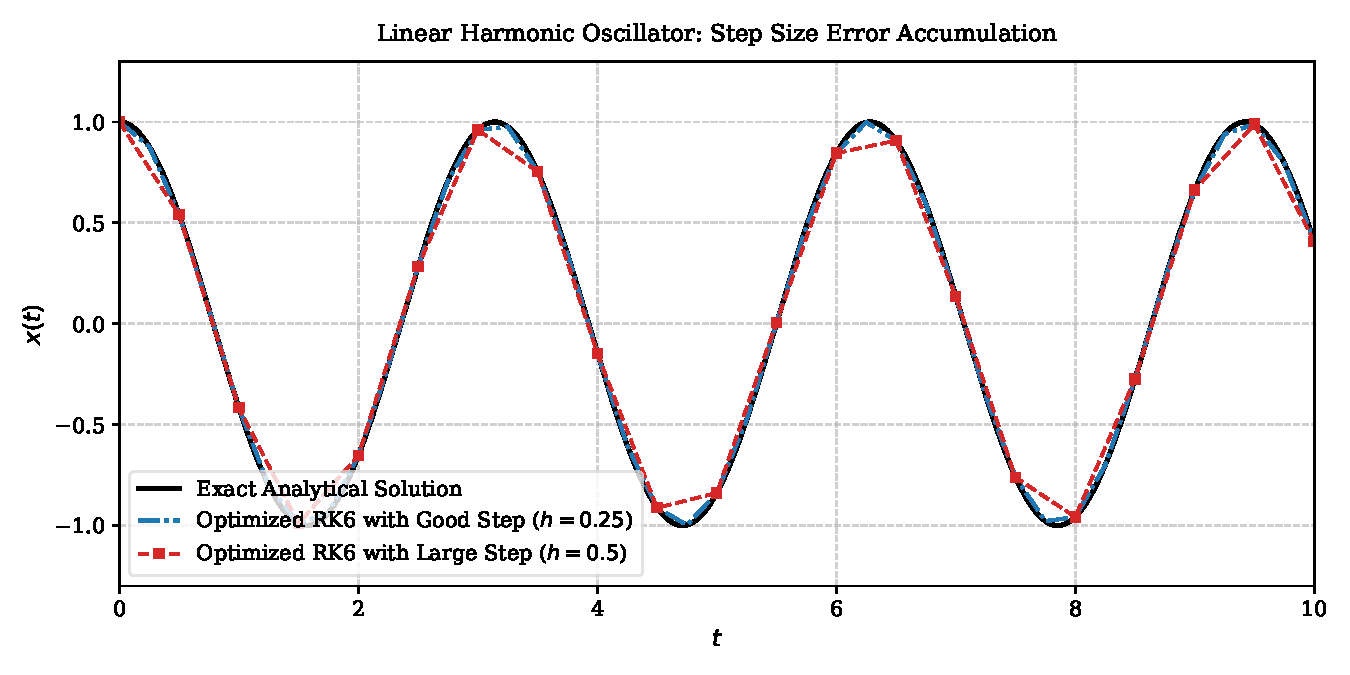
\includegraphics[width=\linewidth]
		{../code/results/visualization/oscillator_visualized}
	\end{figure}
	
\end{frame}